\dev{Emile Martinez}{}

\textit{Cette leçon est là pour présenter vaguement comment interpréter des requêtes SQL}

\begin{com}
	On dessine ces tables au milieu du tableau, et on ne les écrits que quand on en a besoin (car si on les écrits toutes au début c'est long)
\end{com}

\begin{minipage}{0.5\linewidth}
	\begin{center}
		\begin{tabular}{|c|c|c|c|}
			\multicolumn{1}{c}{num\_prod} & \multicolumn{1}{c}{nom} & \multicolumn{1}{c}{prix} & \multicolumn{1}{c}{poids} \\ \hline
			1 & patate & 1 & 1 \\ \hline 
			2 & canard & 8 & 0,4 \\ \hline
			3 & haricots & 4 & 2 \\ \hline
			4 & carottes & 3 & 1,5 \\ \hline
		\end{tabular}\\ \enspace \\
		Table produit
	\end{center}
\end{minipage}
\begin{minipage}{0.5\linewidth}
	\begin{center}
		\begin{tabular}{|c|c|c|}
			\multicolumn{1}{c}{num\_prod} & \multicolumn{1}{c}{num\_client} & \multicolumn{1}{c}{qte}  \\ \hline
			1 & 1 & 3 \\ \hline 
			1 & 2 & 150 \\ \hline
			3 & 1 & 2 \\ \hline
		\end{tabular}\\\enspace\\
		Table commande
	\end{center}
\end{minipage}

\begin{center}
	\begin{tabular}{|c|c|c|c|}
		\multicolumn{1}{c}{num\_client} & \multicolumn{1}{c}{nom} & \multicolumn{1}{c}{adresse} & \multicolumn{1}{c}{ville} \\ \hline
		1 & Radis radieux & 3 allée du swag & Tarbes \\ \hline 
		2 & Navet navigant & 1 allée du caca & Chartres \\ \hline
	\end{tabular}\\ \enspace \\
	Table client
\end{center}

\begin{com}
	Ici commencer par dire : examinons cette requête.
\end{com}

\begin{lstlisting}
<@\textcolor{blue}{SELECT nom, prix}@>
<@\textcolor{red}{FROM produits}@>
<@\textcolor{green}{WHERE poids $>$ 1}@>
\end{lstlisting}

\raisebox{-0.5\height}{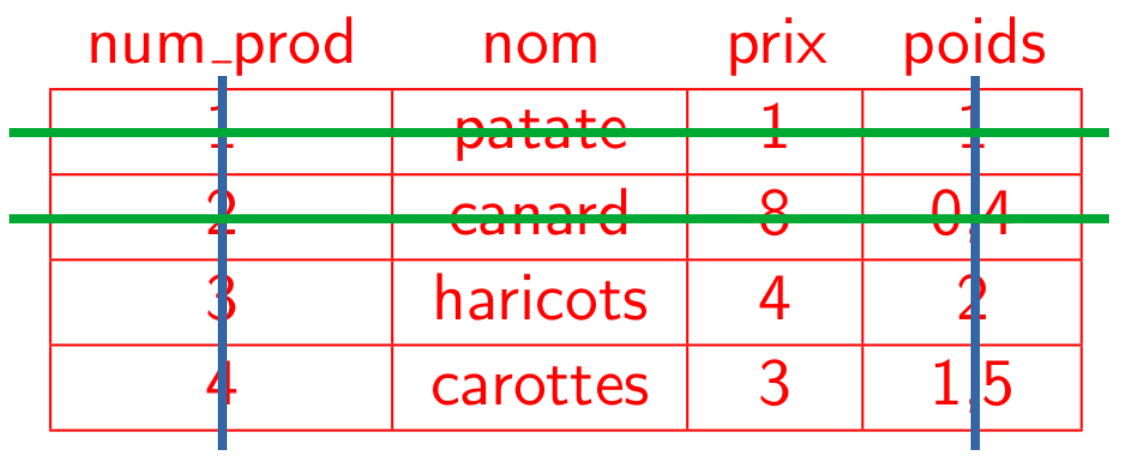
\includegraphics[scale = 0.16]{Developpements/debut sql/exemple1.png}} \qquad $\longrightarrow$ \qquad \begin{tabular}{|c|c|}
	\multicolumn{1}{c}{nom} & \multicolumn{1}{c}{prix} \\ \hline
	haricots & 4 \\ \hline
	carottes & 3 \\ \hline
\end{tabular} 

\begin{com}
	Ca vaut le coup de réécrire la table (même si on mets des abréviations pour les éléments)
\end{com}

On obtient donc les noms et les prix des produits pesant strictement plus de 1 kilo.


\paragraph{Objectif} Afficher les noms des produits de chaque commande avec leur quantité

\begin{lstlisting}
SELECT nom, qte
FROM produit AS p JOIN
commande AS c ON p.num_prod = c.num_prod
\end{lstlisting}

\begin{com}
	La j'écris les premières étapes, à faire évidemment sur le même tableau, et j'élude les dernières. Et expliquez que dans la jointure, on cherche les indices qui correspondent, les entrées qui mettent la condition à vrai
\end{com}

\begin{center}
	
	\begin{tabular}{|c|c|c|c|c|c|c|}
		\hline &&&&&&\\
		&&&&&&\\
	\end{tabular}
	
	$\downarrow$
	
	\begin{tabular}{|c|c|c|c|c|c|c|}
		\hline 1&pat.&1&1&&&\\
		&&&&&&\\
	\end{tabular}
	
	$\downarrow$
	
	\begin{tabular}{|c|c|c|c|c|c|c|}
		\hline 1&pat.&1&1&1&1&3\\
		\hline 1&pat.&1&1&&&\\
		&&&&&&\\
	\end{tabular}
	
	$\downarrow$
	
	\begin{tabular}{|c|c|c|c|c|c|c|}
		\hline 1&pat.&1&1&1&1&3\\
		\hline 1&pat.&1&1&1&2&150\\
		\hline 1&pat.&1&1&&&\\
		&&&&&&\\
	\end{tabular}
	
	$\downarrow$
	
	\begin{tabular}{|c|c|c|c|c|c|c|}
		\hline 1&pat.&1&1&1&1&3\\
		\hline 1&pat.&1&1&1&2&150\\
		\hline 2&can.&8&0,4&&&\\
		&&&&&&\\
	\end{tabular}
	
	$\downarrow$
	
	$\vdots$
	
	$\downarrow$
	
	
	\begin{tabular}{|c|c|c|c|c|c|c|}
		\hline 1&pat.&1&1&1&1&3\\
		\hline 1&pat.&1&1&1&2&150\\
		\hline 3&har.&4&2&3&1&2\\\hline
	\end{tabular}
	
\end{center}

$\longrightarrow$ \qquad \begin{tabular}{|c|c|}
	\multicolumn{1}{c}{nom} & \multicolumn{1}{c}{qte} \\ \hline
	patate & 3 \\ \hline
	patate & 150 \\ \hline
	haricots & 2 \\ \hline
\end{tabular}

\begin{com}
	Là on peut passer sur la droite du tableau (pour avoir d'un côté les requêtes de selection et de l'autre celles d'insertion)
\end{com}


\begin{com}
	Faire les modifications sur la table, en écrivant de la même couleur que la requête
\end{com}
\paragraph{Objectif} Ajouter des commandes


\begin{lstlisting}
<@\textcolor{green}{INSERT INTO commande}@>
<@\textcolor{green}{VALUES (2,2,10), (4,1,1)}@>
\end{lstlisting}

\begin{com}
	Quand on fait ça sur la table, parler de la vérification des conditions faites par SQL
\end{com}

\paragraph{Objectif} Inflation de la patate

\begin{lstlisting}
<@\color{red}UPDATE produit@>
<@\color{red}SET prix = 1.1@>
<@\color{red}WHERE nom = 'patate'@>
\end{lstlisting}

\paragraph{Objectif} Doublement des commandes du client 1

\begin{lstlisting}
<@\color{blue}UPDATE commande@>
<@\color{blue}SET qte = 2*qte@>
<@\color{blue}WHERE num\_client = 1@>
\end{lstlisting}

\paragraph{Objectif} Réalisation de la livraison du produit 1 au client 1

\begin{lstlisting}
<@\color{gray}DELETE FROM commande@>
<@\color{gray} WHERE num\_cient = 1 AND num\_prod = 1@>
\end{lstlisting}

\begin{minipage}{0.5\linewidth}
	\begin{center}
		\begin{tabular}{|c|c|c|c|}
			\multicolumn{1}{c}{num\_prod} & \multicolumn{1}{c}{nom} & \multicolumn{1}{c}{prix} & \multicolumn{1}{c}{poids} \\ \hline
			\rowcolor{gray} 1 & patate & 1 & \sout{1} \color{red} 1,1 \\ \hline 
			2 & canard & 8 & 0,4 \\ \hline
			3 & haricots & 4 & 2 \\ \hline
			4 & carottes & 3 & 1,5 \\ \hline
		\end{tabular}\\ \enspace \\
		Table produit
	\end{center}
\end{minipage}
\begin{minipage}{0.5\linewidth}
	\begin{center}
		\begin{tabular}{|c|c|c|}
			\multicolumn{1}{c}{num\_prod} & \multicolumn{1}{c}{num\_client} & \multicolumn{1}{c}{qte}  \\ \hline
			1 & 1 & \sout 3  \color{blue} 6\\ \hline 
			1 & 2 & 150 \\  \hline
			3 & 1 & \sout 2 \color{blue} 4 \\ \hline
			\color{green} 2 & \color{green} 2 & \color{green} 10\\ \hline
			\color{green} 4 & \color{green} 1 & \sout{\color{green} 1} \color{blue} 2 \\ \hline
		\end{tabular}\\\enspace\\
		Table commande
	\end{center}
\end{minipage}

\paragraph{Une requête plus intéressante} Les noms des produits et des clients qui les commandent, dès que la commande dépassent 10 unités

\begin{lstlisting}
SELECT DISTINCT p.nom, c.nom
FROM produit AS p JOIN
     commande AS co ON co.num_prod = p.num_prod JOIN
     client AS c ON c.num_client = co.num_client
WHERE qte > 10
ORDER BY p.nom ASC
\end{lstlisting}

\begin{rem}
	Le DISTINCT est il utile ?
\end{rem}